% mnras_template.tex
%
% LaTeX template for creating an MNRAS paper
%
% v3.0 released 14 May 2015
% (version numbers match those of mnras.cls)
%
% Copyright (C) Royal Astronomical Society 2015
% Authors:
% Keith T. Smith (Royal Astronomical Society)

% Change log
%
% v3.0 May 2015
%    Renamed to match the new package name
%    Version number matches mnras.cls
%    A few minor tweaks to wording
% v1.0 September 2013
%    Beta testing only - never publicly released
%    First version: a simple (ish) template for creating an MNRAS paper

%%%%%%%%%%%%%%%%%%%%%%%%%%%%%%%%%%%%%%%%%%%%%%%%%%
% Basic setup. Most papers should leave these options alone.
\documentclass[a4paper,fleqn,usenatbib]{mnras}

\usepackage{amsmath}	% Advanced maths commands
% MNRAS is set in Times font. If you don't have this installed (most LaTeX
% installations will be fine) or prefer the old Computer Modern fonts, comment
% out the following line
%\usepackage{newtxtext,newtxmath}
% Depending on your LaTeX fonts installation, you might get better results with one of these:
\usepackage{mathptmx}
\usepackage{txfonts}

% Use vector fonts, so it zooms properly in on-screen viewing software
% Don't change these lines unless you know what you are doing
\usepackage[T1]{fontenc}
\usepackage{ae,aecompl}


%%%%% AUTHORS - PLACE YOUR OWN PACKAGES HERE %%%%%

% Only include extra packages if you really need them. Common packages are:
\usepackage{graphicx}	% Including figure files
%\usepackage{amsmath}	% Advanced maths commands % tady to hazelo errory, presunuti o par radku vys pomohlo, takze pohoda
\usepackage{amssymb}	% Extra maths symbols

%%%%%%%%%%%%%%%%%%%%%%%%%%%%%%%%%%%%%%%%%%%%%%%%%%

%%%%% AUTHORS - PLACE YOUR OWN COMMANDS HERE %%%%%

% Please keep new commands to a minimum, and use \newcommand not \def to avoid
% overwriting existing commands. Example:
%\newcommand{\pcm}{\,cm$^{-2}$}	% per cm-squared

%%%%%%%%%%%%%%%%%%%%%%%%%%%%%%%%%%%%%%%%%%%%%%%%%%

%%%%%%%%%%%%%%%%%%% TITLE PAGE %%%%%%%%%%%%%%%%%%%

% Title of the paper, and the short title which is used in the headers.
% Keep the title short and informative.
\title[Chaos in Bar Potential]{Chaos in Bar Potential}

% The list of authors, and the short list which is used in the headers.
% If you need two or more lines of authors, add an extra line using \newauthor
\author[A. Juranova et al.]{
Anna Juranova;$^{1}$ %\thanks{E-mail: mn@ras.org.uk (KTS)}
mentors: David N. Spergel,$^{2}$
Semyeong Oh$^{2}$
%and Fourth Author$^{3}$
\\
% List of institutions
$^{1}$Department of Theoretical Physics and Astrophysics, Masaryk University, Kotl\'a\v{r}sk\'a 2, 611 37 Brno, Czech Republic\\ %Dept. of Theor. Phys. & Astrophysics; Astronomical Institute, Faculty of Science, Masaryk University, Kotlářská 2, 611 37 Brno, Czech Republic\\
$^{2}$Department of Astrophysical Sciences, Peyton Hall, Princeton University, 4 Ivy Lane, Princeton, NJ USA 08544\\
%$^{3}$Another Department, Different Institution, Street Address, City Postal Code, Country
}

% These dates will be filled out by the publisher
\date{Accepted XXX. Received YYY; in original form ZZZ}

% Enter the current year, for the copyright statements etc.
\pubyear{2016}

% Don't change these lines
\begin{document}
\label{firstpage}
\pagerange{\pageref{firstpage}--\pageref{lastpage}}
\maketitle

% Abstract of the paper
\begin{abstract}
%This is a simple template for authors to write new MNRAS papers.
%The abstract should briefly describe the aims, methods, and main results of the paper.
%It should be a single paragraph not more than 250 words (200 words for Letters).
%No references should appear in the abstract.\\
The amount of chaotic motion in gravitational potential caused by the presence of a galactic bar is closely related to its parameters. Here we aim at quantifying the fraction of chaotic motion as a function of distance from the galactic center, investigating its dependence on the pattern speed and the total mass of the bar. As a model of the bar we use triaxial Ferrers potential, embedded in a composition of a disk, bulge, and dark matter halo models simulating potential of the Milky Way Galaxy. We classify the nature of stellar orbits using Maximum Lyapunov Exponent (MLE) method of chaos detection on a sample of randomly generated orbits within the bar and its close vicinity.\\

\end{abstract}

% Select between one and six entries from the list of approved keywords.
% Don't make up new ones.
\begin{keywords}
galaxies: structure, galaxies: kinematics and dynamics, methods: numerical
\end{keywords}

%%%%%%%%%%%%%%%%%%%%%%%%%%%%%%%%%%%%%%%%%%%%%%%%%%

%%%%%%%%%%%%%%%%% BODY OF PAPER %%%%%%%%%%%%%%%%%%

\section{Introduction}

A large fraction of disc galaxies possess a bar in their central regions, as can be found in \cite{Spitzgal:2015}. These morphological features are accompanied by chaotic orbits, whose presence is given by a lack of axisymmetry in the gravitational potential caused by bars themselves (\cite{BinneyTremaine:2008}. As shown below, spatial distribution of regions supporting chaotic motion and their properties are closely related to the parameters of the potential.

Studying nature of motion in analytic models can widely contribute to our understanding of potential in our own galaxy. Comparing precise information about position and velocities of stars in inner regions with results from analytic modeling, we can put constraints on the form of the potential and its properties. Such information will soon be available from data obtained in GAIA mission.

In this work, we focus on the dependence of a distribution of chaotic orbits in the bar potential on its pattern speed and the total mass. We examine sample of 4000 orbits (4800 orbits in the case of dependence on the mass of the bar) at 20 (24) distances from the center of the potential to its boundaries (and its close vicinity) in the aim to classify them as either regular or chaotic.

\section{Methods and Data}

In this section the model simulating potential of a galaxy is described (Subsect. \ref{sec:potential}) followed by Subsection \ref{sec:chaosdet} briefly explaining the tool used for distinction between regular and chaotic orbits.
%Normally the next section describes the techniques the authors used.
%It is frequently split into subsections, such as Section~\ref{sec:potential} below.

\subsection{Analytical model of the potential}
\label{sec:potential} % used for referring to this section from elsewhere

For the purpose of this work, the bar is represented by a model of Ferrers potential (\cite{Ferrers:1877}). Mass density of this triaxial ellipsoid is given by equation:
\begin{equation} \label{eq:Ferdens}
\rho(\vec{x}) = \left\{
\begin{array}{l l}
\rho_{c}(1-m^{2})^{2}& \quad \textrm{if} \quad m<1,\\
\quad 0& \quad \textrm{if} \quad m \geq 1,\\
\end{array} \right.
\end{equation}
where $\rho_{c}=\frac{105}{32\pi}\frac{G M_{B}}{abc}$ is the central
density, $M_{B}$ is the total mass of the bar and
$m^{2}=\frac{x^{2}}{a^{2}}+\frac{y^{2}}{a^2b^{2}}+\frac{z^{2}}{a^2c^{2}}$,
\mbox{$a>ab>ac> 0$}, with $a,ab$ and $ac$ representing the semi-principal axes of the ellipsoidal
bar. Gravitational constant $ G $ is set to unity. Potential generated by this mass distribution is:

\begin{equation}
	V(\vec{x}) = -\frac{105}{96}G^2\,M_B\,\int_{\lambda}^{\infty} A^{3}(\tau)\,\mathrm{d} \tau
\end{equation}
where
\begin{equation}
	A^{\nu}(\tau) = \frac{\left(1- \sum_{i=1}^{3} \frac{x_i^2}{\tau + a_i^2}\right)^{\nu}}{[(\tau + a^2)(\tau + a^2b^2)(\tau + a^2c^2)]^\frac{1}{2}}
\end{equation}
is part of an integrand which is used again in following equations. Constants and values of parameters of the bar are set according to the final stage of N-body simulation presented in \cite{MachadoManos:2016}. They are listed in Table \ref{tab:potential_params)}. Lower limit for the integral based on definition of the density distribution is given by relation:
\begin{equation}
	\lambda = \begin{cases}
	\text{unique positive solution of} \,\,\, m^2(\lambda)=1, &  \text{for}\ m \geq 1\\
	\lambda = 0\,, & \text{for}\ m < 1
	\end{cases} \\
\end{equation}
where $ m^2(\lambda) = \sum_{i=1}^{3} \frac{x_i^2}{\lambda + a_i^2} $ and $ a_1 = a,\,\,a_2 = ab,\,\,a_3 = ac $.	
The analytical expression of the corresponding
forces is:

\begin{equation}
	F_i = \frac{105}{96}G^2\,M_B\,\frac{b\,c}{2}\, \int_{\lambda}^{\infty} \frac{x_i}{a_i^2 + \tau} A^{2}(\tau)\,\mathrm{d} \tau.
\end{equation}  

%CHECK THE EQUATIONS!

\begin{table}
	\centering
	\caption{Parameters of the Ferrers bar potential used in the model. Semi-major axis $a$ reaches to $ 8\,\mathrm{kpc} $, ratios of semi-principal axes lying in $y$ and $z$ axes are set as $b$ and $c$ values respectively. Pattern speed $\Omega_B$ and the bar mass $M_B$ vary for different cases we examine and lie in listed intervals.}
	\label{tab:potential_params)}
	\begin{tabular}{cc} % four columns, alignment for each
		\hline
		Parameter & Value \\
		\hline
		$ a $ & $8\,\mathrm{kpc}$\\
		$ b $ & $ 0.35 $\\
		$ c $ & $ 0.2375 $\\
		$ \Omega_B $ & $ \left< 10;27.5\right>\,\mathrm{km/s/kpc} $\\
		$ M_{B} $ & $ \left<8.25;16.5\right>\, \times 10^{9} M_{\odot}$\\
		\hline
	\end{tabular}
\end{table}

The bar potential is embedded in a model of Milky Way galaxy potential provided in \textit{galpy} package written in Python programming language (\cite{Bovy:2015}). The Milky Way model is a composition of Miyamoto-Nagai potential (\ref{eq:disk}) for disk \cite{MiyamotoNagai:1975}, NFW profile (\ref{eq:halo}) for the dark matter halo \cite{NFW:1996} and exponentially cut-off power-law density profile (\ref{eq:bulge}) component for a spherical bulge. Parameters of these components are shown in Table \ref{tab:MWpot_params}, further details can be found in \cite{Bovy:2015}.

\begin{equation}\label{eq:bulge}
	\rho_b(r)=\rho_0 \, \left(  \frac{r_0}{r} \right) ^{\alpha} \exp -\left( \frac{r}{r_c} \right)^2
\end{equation}

\begin{equation}\label{eq:disk}
	\Phi_d(R,z) = -\frac{GM_d}{\sqrt{R^2+(a+\sqrt{z^2+b^2})^2}}\\
\end{equation}

\begin{equation}\label{eq:halo}
	\rho_h(r) = \frac{GM_h}{4\,\pi\,R_s^3}\,\frac{1}{(r/R_s)\,(1+r/R_s)^{2}}\\
\end{equation}

\begin{table}
	\centering
	\caption{Parameters of the Milky Way-like model of potential. Values denoted as $ f $ stand for the fraction of radial force in galactic plane at solar radius $ R_0 $.}
	\label{tab:MWpot_params}
	\begin{tabular}{lcc} % alignment for each column
		\hline
		Component & Parameter		 		& Value \\
		\hline
		\hline
			 	&$ R_0 $			 		& $ 8				\,\mathrm{kpc} $\\
				&$ v_c(R_0) $		 		& $ 220				\,\mathrm{km/s} $\\
		\hline
		\hline
		Bulge 	&$ \alpha $				& $ -1.8			 $\\
				&$ r_c $ 					& $ 1.9				\,\mathrm{kpc} $\\
				&$ f_b $			 		& $ 0.05			 $\\
				&$ M_{b} $		 			& $ 5\times 10^{9} 	\,M_{\odot} $\\
		\hline
		Disk	&$ a $			 			& $ 3.0				\,\mathrm{kpc} $\\
				&$ b $			 			& $ 280				\,\mathrm{pc} $\\
				&$ f_d $			 		& $ 0.60			 $\\
				&$ M_{d} $		 			& $ 6.8\times 10^{10}\,M_{\odot} $\\
		\hline
		Halo	&$ R_s $	 				& $ 16				\,\mathrm{kpc} $\\
				&$ \rho_{DM}(R_0) $ 		& $ 0.008			\,M_{\odot}\mathrm{pc^{-3}} $\\
				&$ f_{h} $ 					& $ 0.35			\,\mathrm{kpc} $\\
				&$ M_{h} $		 			& $	3.27			\,\times 10^{11} M_{\odot}$\\
%		$ \sigma_b $	 					& $ 109				\,\mathrm{km/s} $\\
%		$ F_z(R_0, z = 1.1\,\mathrm{kpc}) $ & $ 72\times2\pi G	\,\mathrm{M_\odot pc^{-2}} $\\
%		$ \Sigma_{vis}(R_0) $ 				& $ 53				\,\mathrm{M_\odot pc^{-2}} $\\
%		$ F_z $ scale length 				& $ 3.2				\,\mathrm{kpc} $\\
%		$ \rho (R_0, z = 0\,\mathrm{kpc}) $ & $ 0.10			\,\mathrm{M_{\odot}pc^{-3}} $\\
%		$ (d \ln(v_c/d)\ln (R))(R_0) $ 		& $ -0.10			 $\\
%		$ M(r<60\,\mathrm{kpc}) $ 			& $ 4.1\times 10^{11}\,\mathrm{M_{\odot}} $\\
%		$ R_{d} $							& $ 2.6				\,\mathrm{kpc} $\\
%		$ M_{vir} $		 					& $ 0.8\times 10^{9}\,\mathrm{M_{\odot}} $\\
%		$ r_{vir} $		 					& $ 245				\,\mathrm{kpc} $\\
%		$ \mathrm{Concentration} $ 			& $ 15.3			 $\\
%		$ v_{esc}(R_0) $ 					& $ 513				\,\mathrm{km/s}$\\
		\hline
	\end{tabular}
\end{table}

\subsection{Chaos detection method}
\label{sec:chaosdet}
Various chaos detection methods exist, taking advantage of main differences between regular and chaotic orbits, f.e. frequency diffusion rate described in \cite{APW_SuperFreq:2016} or techniques based on behavior in phase space to be found in \cite{Skokos_GALI:2007,SkokosManos_GALI_SALI:2014}.

Chaos detection method used here belongs to the category mentioned later. The Maximum Lyapunov Exponent (MLE) method is based on a fact that chaotic motion is expressed by an exponential divergence of close orbits. Its main advantage among other techniques in this category is its simplicity and lower computational cost. Following paragraphs are dedicated to its definition and computation for 3-d.o.f. Hamiltonian function for the motion of a star in a 3 dimensional rotating barred galaxy:
\begin{equation}\label{eq:Hamilton}
	H=\frac{1}{2} (p_{x}^{2}+p_{y}^{2}+p_{z}^{2})+ V(x,y,z,t) -
	\Omega_B (xp_{y}-yp_{x}).
\end{equation}
Pattern speed $ \Omega_B $ is an angular velocity of the bar around z-axis ($ \vec{\Omega}_b = \hat{e}_z\,\Omega_b $), the shortest principal axis, the $x$ direction is along the major axis and the $y$ along the intermediate axis of the bar. The $p_{x}$, $p_{y}$ and $p_{z}$ are the canonically conjugate momenta, $V$ is the potential, and $H$ is the total energy of the orbit in the rotating frame of reference.\\
Equations of motion in this potential are:
\begin{equation}\label{eq:motion}
	\begin{array}{lcl}
	\dot{x} &=& \displaystyle p_{x} + \Omega_B y, \\
	\dot{y} &=& \displaystyle p_{y} - \Omega_B x,  \\
	\dot{z} &=& \displaystyle p_{z}, \\
	\dot{p_{x}} &=& \displaystyle -\frac{\partial V}{\partial x} + \Omega_B p_{y}, \\
	\dot{p_{y}} &=& \displaystyle -\frac{\partial V}{\partial y} - \Omega_B p_{x}, \\
	\dot{p_{z}} & =& \displaystyle -\frac{\partial V}{\partial z}. \\
	\end{array}
\end{equation}
Information about evolution of separation of any two initially infinitesimally close orbits described by deviation vector $\mathbf{w}=(\delta x,\delta y,\delta z,\delta p_{x},\delta p_{y},\delta
p_{z})$ needs to be known for the calculation of the MLE. Equations of motion for $\mathbf{w}$ are given by the
variational equations:
\begin{equation}\label{eq:dev_vect}
	\begin{array}{lcl}
	\dot{\delta x} &=& \displaystyle \delta p_{x} + \Omega_B \delta y,  \\
	\dot{\delta y} &=& \displaystyle \delta p_{y} + \Omega_B \delta x,  \\
	\dot{\delta z} &=& \displaystyle\delta p_{z},\\
	\dot{\delta p_{x}} &=& \displaystyle- \frac{\partial^2 V}{\partial x \partial x}\delta x -
	\frac{\partial^2 V}{\partial x \partial y}\delta
	y - \frac{\partial^2 V}{\partial x \partial z} \delta z + \Omega_B \delta p_{y}, \\
	\dot{\delta p_{y}} &=& \displaystyle- \frac{\partial^2 V}{\partial y \partial x}\delta x -
	\frac{\partial^2 V}{\partial y \partial y}\delta
	y - \frac{\partial^2 V}{\partial y \partial z} \delta z - \Omega_B \delta p_{x}, \\
	\dot{\delta p_{z}} &=& \displaystyle- \frac{\partial^2 V}{\partial z \partial x}\delta x -
	\frac{\partial^2 V}{\partial z \partial y}\delta y - \frac{\partial^2 V}{\partial z \partial z} \delta z. \\
	\end{array}
\end{equation}

In order to compute the value of MLE, both sets of equations (time-dependent set of ordinary differential equations (\ref{eq:motion}) and (\ref{eq:dev_vect})) need to be solved simultaneously. This requirement arises from the fact that derivatives of the rotating potential depend explicitly on time and (\ref{eq:motion}) are therefore non-autonomous.
As described in \cite{BinneyTremaine:2008,APW_SuperFreq:2016} in further details, the MLE value $ \lambda_i $ is defined as:
\begin{equation}
	\label{LE}
	\lambda_i =\lim_{t \rightarrow \infty} \sigma_i(t),
\end{equation}
where:
\begin{equation}
	\label{sigma_i}
	\sigma_i(t)= \frac{1}{t}
	\ln \frac{\|\mathbf{w}(t)\|}{\|\mathbf{w}(0)\|}.
\end{equation}
For obvious practical reasons, it is feasible to use approximation for finite time, the so-called 'finite time MLE' (\ref{eq:finite_time_MLE}), for which $\|\mathbf{w}(0)\|$ and $\|\mathbf{w}(t_i)\|$ are the Euclidean norms of the deviation vector at times
$t=0$ and $t>0$ respectively.
\begin{equation}\label{eq:finite_time_MLE}
	\lambda_N = \frac{1}{t_N} \sum_{i}^{N} \ln \frac{|| \delta \textbf{w}(t_i)||}{||\delta \textbf{w} _0||}
\end{equation}

Examining the evolution of the $ \sigma_i $ in time, we can distinguish between regular and chaotic orbits based on the general trend: for regular motion, the value tends to zero following power law, whereas in the latter case, the value converges to a positive value allowing the deviation vector to increase exponentially.
%Should I describe computation of the Lyapunov exponent in practise?

\subsection{Data generation and analysis}

To analyze the fraction of chaos in our potential, we generated a sample of 4000 initial conditions for orbits starting at galactic plane, with uniformly distributed components of velocity vectors. Each subsample constituting of 200 orbits has specific apocentric distance within the bar and is analyzed individually. Orbits are integrated for 20\,Gy using leapfrog integrator described in \cite{BinneyTremaine:2008}, mainly for sufficient conservation of energy.

Having finite-time MLEs calculated for each sample, the final classification of orbits is based on the final value of MLE. Sufficiently long integration time allows using reasonably set threshold value to distinguish between each type. For a typical example of chaotic orbit the value differs from the one for regular orbit in order of two magnitudes. Validity of this step was confirmed during visual inspection of the descending trend described in \ref{sec:chaosdet}.
%Should I mention that galpy was used for the integration again?

\section{Discussion}
In this section, we present results of examining the nature of orbits in the potential having different values of total mass and pattern speed. Motion in each potential was tested for 200 orbits per each apocentric radius -- each point in the plot. 

\subsection{Dependence on total mass}
Chaotic orbits populating sphere at the maximal distance being 1.2 times semi-major axis of the ellipsoidal bar were tested for two general cases different in the total mass of the bar. The amount of chaos present in potential including the bar of total mass $ 33\times 10^9\, M_{\odot} $ is shown in Fig. \ref{fig:total_mass} along with curve presenting the same for less massive bar ($ M_B = 16.5\,\times 10^9\, M_{\odot} $). As expected, the bar-induced chaoticity is more significant in the former case, where the overall fraction of chaos is approximately 73\,\%, whereas for the latter it is about 10\,\% less. The pattern speed in both cases was set to be $ 10\,\mathrm{km/s/kpc} $. Comparing the results with ones from \cite{MachadoManos:2016}, the amount is rather high with similar parameters of the bar, yet embedded in slightly different potential which stands for remaining morphological features of the galaxy.

\begin{figure}
	% Allowable file formats are eps or ps if compiling using latex
	% or pdf, png, jpg if compiling using pdflatex
	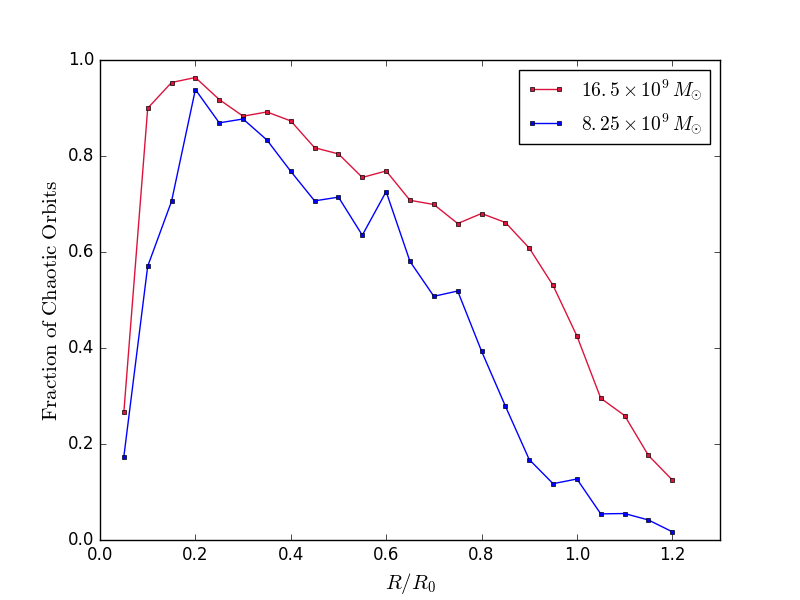
\includegraphics[width=\columnwidth]{mass_dep}
	\caption{Relative amount of chaos shown as a function of distance from the center of the potential model with Ferrers bar rotating at $ \Omega_B = 10.0\,\mathrm{km/s/kpc} $ for two cases, where the total mass of the bar is (a) $ 33 \times 10^9 M_{\odot}$ (red curve); (b) $ 16.5 \times 10^9\,M_{\odot}$ (blue curve), half of the former. $ R_0 = 8\,\mathrm{kpc} $ and is equal to size of semi-major axis of the bar.}
	\label{fig:total_mass}
\end{figure}

\subsection{Dependence on pattern speed}
As $ 10\,\mathrm{km/s/kpc} $ is rather low pattern speed compared to what is expected to be found in the Galaxy, we examined how the situation changes for higher values of $ \Omega_B $. In Fig. \ref{fig:pattern_speed} the fraction of chaoticity as a function of apocentric distance of an object is shown for five pattern speeds starting at $ 10\,\mathrm{km/s/kpc} $ up to angular velocity at which the stars at solar distance corrotate with the bar.

The obvious general trend is that the area mostly populated by chaotic orbits in central parts of the bar weakens in favor of chaoticity increase in outer regions. The overall amount of chaos remains practically constant and around 60\,\%. However, there are some observable inconsistencies in the plot, f.e. in case of the curve with pattern speed of $ 23.1\,\mathrm{km/s/kpc} $. The explanation for such discrepancies most probably lies in an insufficient number of orbits tested in the study.
 
\begin{figure}
	% Allowable file formats are eps or ps if compiling using latex
	% or pdf, png, jpg if compiling using pdflatex
	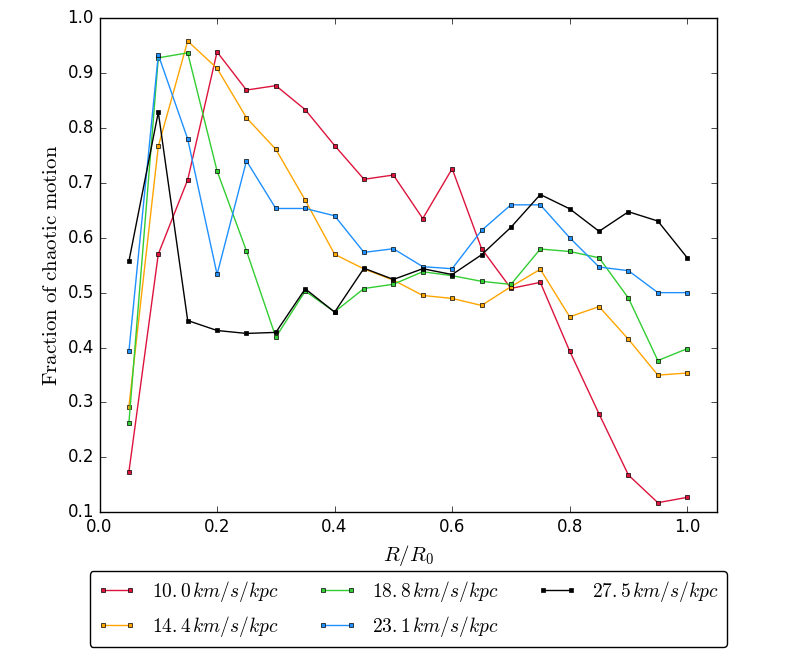
\includegraphics[width=\columnwidth]{all3}
	\caption{Fraction of chaotic orbits presented as a function of radius for potential with the Ferrers bar rotating at different pattern speeds. The maximum speed of $ 27.5\,\mathrm{km/s/kpc} $ is the corrotation velocity of Sun at distance $ R_0 = 8\,\mathrm{kpc} $ ($ v_0(R_0) = 220\,\mathrm{km/s}$). Mass of the bar for all five curves is $ 8.25\times 10^{9}\,\mathrm{M_{\odot}} $.}
	\label{fig:pattern_speed}
\end{figure}


%\subsection{Figures and tables}

%Figures and tables should be placed at logical positions in the text. Don't
%worry about the exact layout, which will be handled by the publishers.

%Figures are referred to as e.g. Fig.~\ref{fig:example_figure}, and tables as
%e.g. Table~\ref{tab:example_table}.

% Example figure
%\begin{figure}
	% To include a figure from a file named example.*
	% Allowable file formats are eps or ps if compiling using latex
	% or pdf, png, jpg if compiling using pdflatex
%	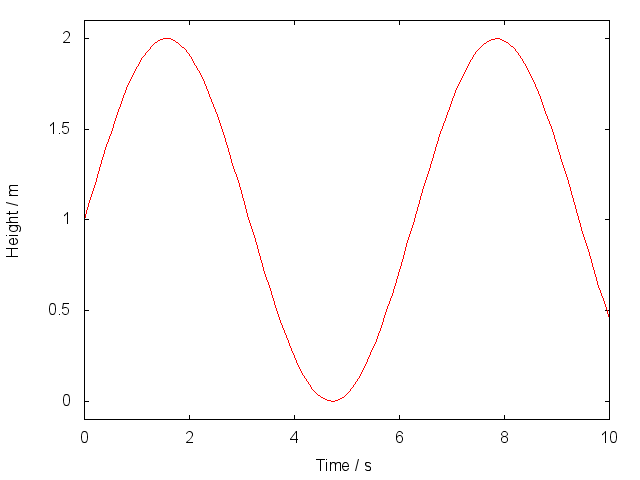
\includegraphics[width=\columnwidth]{example}
%    \caption{This is an example figure. Captions appear below each figure.
%	Give enough detail for the reader to understand what they're looking at,
%	but leave detailed discussion to the main body of the text.}
%    \label{fig:example_figure}
%\end{figure}

% Example table
%\begin{table}
%	\centering
%	\caption{This is an example table. Captions appear above each table.
%	Remember to define the quantities, symbols and units used.}
%	\label{tab:example_table}
%	\begin{tabular}{lccr} % four columns, alignment for each
%		\hline
%		A & B & C & D\\
%		\hline
%		1 & 2 & 3 & 4\\
%		2 & 4 & 6 & 8\\
%		3 & 5 & 7 & 9\\
%		\hline
%	\end{tabular}
%\end{table}


\section{Summary and conclusions}

We performed an analysis of stellar motion in a bar potential embedded in central part of a realistic model of a galaxy to explore the amount of chaos present and to describe its dependence on basic properties of the bar potential.

Using Ferrers potential as a model of a galactic bar, we focused on studying the fraction of chaotic motion as a function of apocentric radius of tested orbits and its dependence on total mass and the pattern speed of the bar. For classification of an orbit as either regular or chaotic, we used Maximum Lyapunov Exponent method for being the most convenient for this work, considering computational demands of the orbit integration.

Rather expected overall decrease of chaos when having lower massive bar was measured with confidence. The change of chaotic orbits distribution for varying pattern speed was also obvious from the data, supporting the idea that information obtained when studying these analytical objects can be valuable when giving constraints on the actual form of the potential. However, we should keep in mind that models represented by triaxial ellipsoid are a poor approximation of real shapes of galactic bars.  
\\

%The last numbered section should briefly summarise what has been done, and describe
%the final conclusions which the authors draw from their work.

\section*{Acknowledgements}

I would like to express my gratitude to David Spergel and Semyeong Oh for their time and patient guidance throughout this project and to Adrian Price-Whelan for his assistance and helpful advice. I would also like to thank the USRP Organizing Committee for giving me the opportunity to participate in this wonderful summer program and to the Department of Astrophysical Sciences of Princeton University for providing us all the facilities needed for our research.
 
%The Acknowledgements section is not numbered. Here you can thank helpful
%colleagues, acknowledge funding agencies, telescopes and facilities used etc.
%Try to keep it short.

%%%%%%%%%%%%%%%%%%%%%%%%%%%%%%%%%%%%%%%%%%%%%%%%%%

%%%%%%%%%%%%%%%%%%%% REFERENCES %%%%%%%%%%%%%%%%%%

% The best way to enter references is to use BibTeX:
%\nocite{*}
\bibliographystyle{mnras}
\bibliography{report} % if your bibtex file is called example.bib


%%%%%%%%%%%%%%%%%%%%%%%%%%%%%%%%%%%%%%%%%%%%%%%%%%

%%%%%%%%%%%%%%%%% APPENDICES %%%%%%%%%%%%%%%%%%%%%

%\appendix

%\section{Some extra material}

%If you want to present additional material which would interrupt the flow of the main paper,
%it can be placed in an Appendix which appears after the list of references.

%%%%%%%%%%%%%%%%%%%%%%%%%%%%%%%%%%%%%%%%%%%%%%%%%%


% Don't change these lines
\bsp	% typesetting comment
\label{lastpage}
\end{document}

% End of mnras_template.tex